% MFA Client Authentication — User Guide
% Compile: pdflatex userguide.tex  (run twice for TOC)
% Location: MFA_Client_Authentication/docs/

\documentclass[11pt,a4paper]{article}

\usepackage[margin=2.5cm]{geometry}
\usepackage[T1]{fontenc}
\usepackage{lmodern}
\usepackage{microtype}
\usepackage{amsmath}
\usepackage{booktabs}
\usepackage{hyperref}
\usepackage{xcolor}
\usepackage{tikz}
\usepackage{enumitem}
\usepackage{listings}
\usetikzlibrary{arrows.meta, positioning, fit, backgrounds, calc}

\hypersetup{
  colorlinks=true,
  linkcolor=blue!60!black,
  urlcolor=blue!60!black,
  pdftitle={MFA Client Authentication User Guide},
  pdfauthor={Secure Banking Project}
}

\definecolor{accent}{RGB}{40,80,120}
\definecolor{pcbox}{RGB}{210,230,255}
\definecolor{espbox}{RGB}{220,245,220}
\definecolor{warnbox}{RGB}{255,240,210}
\definecolor{codebg}{RGB}{248,248,248}

\lstset{
  basicstyle=\ttfamily\small,
  backgroundcolor=\color{codebg},
  frame=single,
  framerule=0.4pt,
  breaklines=true,
  columns=fullflexible,
  showstringspaces=false,
  aboveskip=0.6em,
  belowskip=0.4em,
}

\newcommand{\code}[1]{\texttt{#1}}
\newcommand{\filepath}[1]{\texttt{\detokenize{#1}}}

\title{%
  \textbf{MFA Client Authentication}\\[0.35em]
  \large User Guide for New Users\\
  \normalsize Secure Banking --- ESP32-C6 + Windows PC
}
\author{Secure Banking Project}
\date{\today}

\begin{document}
\maketitle

\begin{abstract}
This folder implements a \textbf{two-factor net-banking login demo}:
something you know (password on the PC) plus something you have (a PUF-backed
hardware token on ESP32-C6). The raw PUF secret never leaves the chip; the PC
only receives a cryptographic proof over USB serial. This guide walks a new user
through setup, daily use, and troubleshooting.
\end{abstract}

\tableofcontents
\newpage

%==============================================================================
\section{What This Project Does}
%==============================================================================

The \filepath{MFA\_Client\_Authentication/} folder is a complete lab stack for
\textbf{PUF-rooted multi-factor authentication (MFA)} over UART:

\begin{itemize}[noitemsep]
  \item \textbf{ESP32 side} (\filepath{esp32/}): reads the chip PUF at boot,
        derives a device X25519 key, and answers MFA commands on USB serial.
  \item \textbf{PC side} (\filepath{pc/}): simulates a bank login page, checks
        a password, then challenges the hardware device and verifies its response.
\end{itemize}

This is \textbf{not} production banking software. It demonstrates the
architecture: password + hardware MFA, with keys rooted in silicon.

\subsection{The three layers you must complete}

\begin{center}
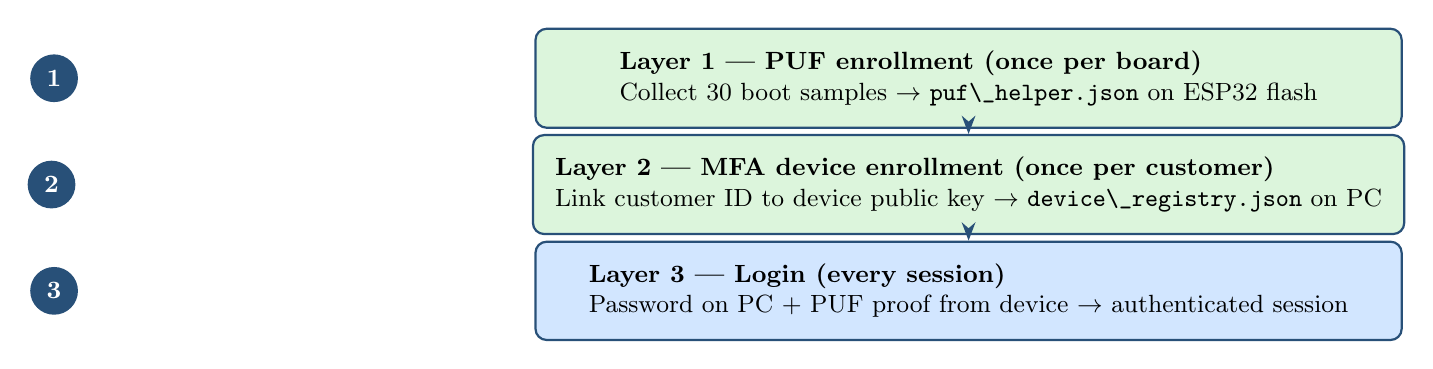
\begin{tikzpicture}[
  layer/.style={
    draw=accent, thick, rounded corners=4pt,
    minimum width=11cm, minimum height=0.95cm,
    align=left, inner sep=8pt, font=\small
  },
  num/.style={circle, fill=accent, text=white, font=\bfseries\small, minimum size=6mm}
]
  \node[layer, fill=espbox] (l1) at (0,0) {
    \textbf{Layer 1 --- PUF enrollment (once per board)}\\
    Collect 30 boot samples $\rightarrow$ \filepath{puf\_helper.json} on ESP32 flash
  };
  \node[layer, fill=espbox] (l2) at (0,-1.35) {
    \textbf{Layer 2 --- MFA device enrollment (once per customer)}\\
    Link customer ID to device public key $\rightarrow$ \filepath{device\_registry.json} on PC
  };
  \node[layer, fill=pcbox] (l3) at (0,-2.7) {
    \textbf{Layer 3 --- Login (every session)}\\
    Password on PC + PUF proof from device $\rightarrow$ authenticated session
  };

  \node[num] at ([xshift=-6.1cm]l1.west) {1};
  \node[num] at ([xshift=-6.1cm]l2.west) {2};
  \node[num] at ([xshift=-6.1cm]l3.west) {3};

  \draw[-{Stealth}, thick, accent] (l1.south) -- (l2.north);
  \draw[-{Stealth}, thick, accent] (l2.south) -- (l3.north);
\end{tikzpicture}
\end{center}

Layer~1 uses the PUF enrollment script in \filepath{Code/main.py} (parent project).
Layers~2 and~3 use this folder's \filepath{pc/} clients and \filepath{esp32/main.py}.

%==============================================================================
\section{What You Need}
%==============================================================================

\subsection{Hardware}

\begin{itemize}
  \item ESP32-C6 development board with USB serial (example: COM5 on Windows)
  \item USB cable; note the correct COM port in Device Manager
  \item Windows PC (this guide uses PowerShell-style paths; Linux/macOS work with \code{/dev/tty*} ports)
\end{itemize}

\subsection{Software}

\begin{table}[h]
  \centering
  \caption{Required software}
  \begin{tabular}{@{}llp{5.5cm}@{}}
    \toprule
    \textbf{Component} & \textbf{Where} & \textbf{Purpose} \\
    \midrule
    MicroPython (ESP32-C6) & On the board & Runs \filepath{boot.py} + \filepath{main.py} \\
    Thonny or \code{mpremote} & PC & Flash \filepath{.py} files to ESP32 \\
    Python 3.8+ & PC & Run enrollment and login clients \\
    \code{pyserial} & PC & USB serial communication \\
    \LaTeX{} (optional) & PC & Build this PDF from \filepath{userguide.tex} \\
    \bottomrule
  \end{tabular}
\end{table}

\subsection{Install PC dependencies}

From the \filepath{pc/} directory:

\begin{lstlisting}
cd MFA_Client_Authentication\pc
pip install -r requirements.txt
\end{lstlisting}

Only \code{pyserial} is required for the lab clients.

%==============================================================================
\section{Folder Layout}
%==============================================================================

\begin{verbatim}
MFA_Client_Authentication/
├── docs/
│   └── userguide.tex          <- this document
├── esp32/                     <- copy ALL .py files to the board
│   ├── boot.py                <- reads LP-SRAM PUF once per boot
│   ├── main.py                <- MFA UART server (run after PUF enrolled)
│   ├── key_derive.py          <- PUF reconstruct + HKDF
│   ├── device_identity.py     <- PUF-rooted X25519 key
│   ├── mfa_auth.py            <- login HMAC proof
│   ├── mfa_store.py           <- mfa_enrollment.json on flash
│   ├── mfa_protocol.py        <- UART command constants
│   ├── puf_io.py, sketch.py, bch.py, hkdf.py, x25519.py, ...
│   └── config.py              <- baud rate, file paths, HKDF labels
└── pc/
    ├── enroll_client.py       <- register device for a customer
    ├── login_client.py        <- password + device MFA login
    ├── uart_client.py         <- serial helpers
    ├── protocol.py            <- parse MFA responses
    ├── mfa_auth.py              <- verify HMAC proof
    ├── x25519_pure.py         <- must match ESP X25519 math
    ├── device_registry.json   <- bank-side device records
    └── requirements.txt
\end{verbatim}

\textbf{Rule of thumb:} everything under \filepath{esp32/*.py} goes on the chip;
everything under \filepath{pc/} stays on the computer.

%==============================================================================
\section{End-to-End Architecture}
%==============================================================================

\begin{center}
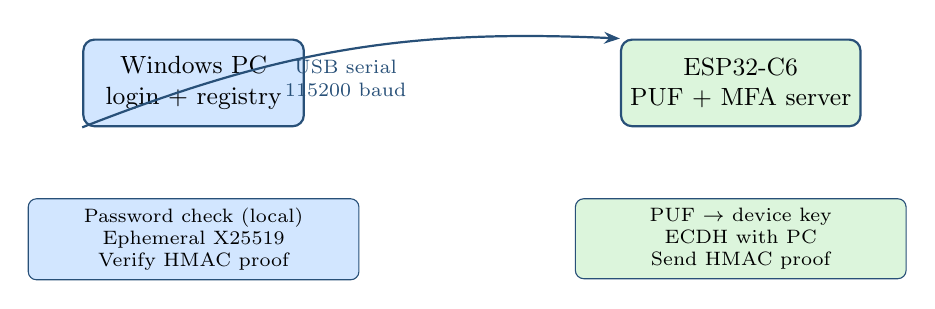
\begin{tikzpicture}[
  actor/.style={
    draw=accent, thick, rounded corners=4pt,
    minimum width=2.8cm, minimum height=1.1cm, align=center, font=\small
  },
  arr/.style={-{Stealth[length=2mm]}, thick, accent},
  lbl/.style={font=\scriptsize, align=center}
]
  \node[actor, fill=pcbox] (pc) {Windows PC\\login + registry};
  \node[actor, fill=espbox, right=4cm of pc] (esp) {ESP32-C6\\PUF + MFA server};

  \draw[arr] (pc.south west) to[bend left=12]
    node[lbl, below]{USB serial\\115200 baud} (esp.north west);

  \node[below=0.9cm of pc, draw=accent, rounded corners=3pt, fill=pcbox,
    minimum width=4.2cm, align=center, font=\scriptsize] {
    Password check (local)\\Ephemeral X25519\\Verify HMAC proof
  };
  \node[below=0.9cm of esp, draw=accent, rounded corners=3pt, fill=espbox,
    minimum width=4.2cm, align=center, font=\scriptsize] {
    PUF $\rightarrow$ device key\\ECDH with PC\\Send HMAC proof
  };
\end{tikzpicture}
\end{center}

\textbf{Never sent over the wire:} raw PUF data, stable PUF word, device private
scalar, or the final PUF-derived AES key.

\textbf{Sent over the wire:} protocol text lines (status, enroll, auth challenge,
HMAC proof). The PC learns only the device \emph{public} key at enrollment time.

%==============================================================================
\section{Step-by-Step Setup}
%==============================================================================

\subsection{Step 1: PUF enrollment on the ESP32 (Layer 1)}

Before MFA works, the board must complete \textbf{PUF fuzzy extraction enrollment}.
This is a \textbf{one-time} process per physical chip.

\begin{enumerate}
  \item Copy PUF stack files to the board: at minimum \filepath{boot.py},
        \filepath{puf\_state.py}, \filepath{puf\_io.py}, \filepath{bch.py},
        \filepath{sketch.py}, \filepath{hkdf.py}, \filepath{config.py}, and
        \textbf{\filepath{Code/main.py}} from the parent project (rename or use
        as \filepath{main.py} on the board).
  \item Reset the board. Each boot appends one LP-SRAM sample.
  \item \textbf{Power-cycle 30 times} (\code{ENROLL\_SAMPLES = 30}). Watch serial
        output: \code{sample 1/30}, \code{2/30}, \ldots
  \item After sample 30, enrollment finalises and writes:
        \begin{itemize}
          \item \filepath{/puf\_helper.json} --- stable bit positions, BCH syndrome, salt
          \item \filepath{/.puf\_enrolled} --- marker file
        \end{itemize}
  \item Confirm serial shows \code{=== ENROLLMENT COMPLETE ===}.
\end{enumerate}

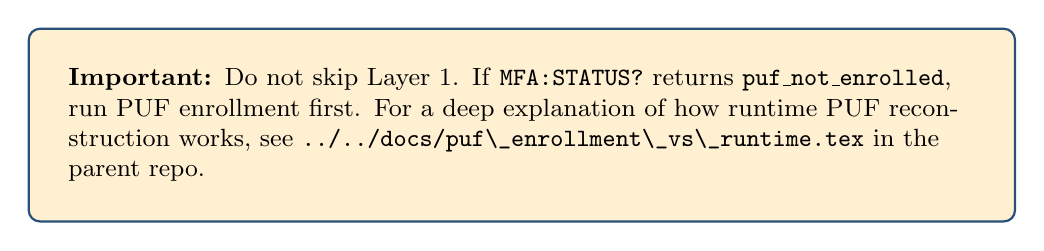
\begin{tikzpicture}[framed, background rectangle/.style={fill=warnbox, draw=accent, thick, rounded corners=4pt}]
  \node[inner sep=10pt, font=\small, text width=0.95\linewidth] {
    \textbf{Important:} Do not skip Layer~1. If \filepath{MFA:STATUS?} returns
    \code{puf\_not\_enrolled}, run PUF enrollment first. For a deep explanation of
    how runtime PUF reconstruction works, see
    \filepath{../../docs/puf\_enrollment\_vs\_runtime.tex} in the parent repo.
  };
\end{tikzpicture}

\subsection{Step 2: Deploy the MFA server (replace \filepath{main.py})}

After PUF enrollment succeeds:

\begin{enumerate}
  \item \textbf{Keep} on the board: \filepath{boot.py}, \filepath{puf\_helper.json},
        \filepath{.puf\_enrolled}, and all crypto modules from \filepath{esp32/}.
  \item \textbf{Replace} \filepath{main.py} with
        \filepath{MFA\_Client\_Authentication/esp32/main.py}.
  \item \textbf{Remove} conflicting files from other demos if present (e.g.\
        \filepath{pairing.json}, \filepath{secure\_protocol.py} from the secure UART demo).
  \item Reset the board. Serial should show:
\begin{lstlisting}
MFA PUF device server  baud=115200
Status: puf_ready
\end{lstlisting}
  \item Close Thonny or any serial monitor before running PC clients (only one
        program may open the COM port).
\end{enumerate}

\subsection{Step 3: List serial ports (optional)}

\begin{lstlisting}
python enroll_client.py --list-ports
\end{lstlisting}

Use the port name shown (e.g.\ \code{COM5}) in the next steps.

\subsection{Step 4: MFA device enrollment (Layer 2)}

Link a bank customer ID to this physical device:

\begin{lstlisting}
cd MFA_Client_Authentication\pc
python enroll_client.py --port COM5 --customer CUST10042
\end{lstlisting}

Expected output:

\begin{lstlisting}
Connected to COM5
Device status: puf_ready
Enrolling customer CUST10042 ...
Enrollment OK
  Customer   : CUST10042
  Device pubkey: 6e75b5b8e10c3c2f6746959ff7337ee ...
  Saved to   : device_registry.json
\end{lstlisting}

The PC stores the mapping in \filepath{device\_registry.json}. The ESP32 stores
\filepath{/mfa\_enrollment.json} with the same customer ID and public key hex.

After this, \code{MFA:STATUS?} should return \code{mfa\_enrolled}.

\subsection{Step 5: Login with password + device MFA (Layer 3)}

\begin{lstlisting}
python login_client.py --port COM5 --customer CUST10042 --password demo1234
\end{lstlisting}

Add \code{--verbose} to see every serial line. Authentication on the device
(PUF + X25519) may take \textbf{several seconds} on ESP32-C6; the client waits up
to 120\,s.

Successful login ends with:

\begin{lstlisting}
=== LOGIN SUCCESS ===
Factors: password + PUF hardware device
Customer: CUST10042
Session : LOGIN-xxxxxxxx
\end{lstlisting}

%==============================================================================
\section{What Happens During Login}
%==============================================================================

\subsection{Two factors}

\begin{table}[h]
  \centering
  \caption{Authentication factors in this lab}
  \begin{tabular}{@{}lll@{}}
    \toprule
    \textbf{Factor} & \textbf{Where} & \textbf{In this demo} \\
    \midrule
    Something you know & PC & Password (\code{--password}, min.\ 4 chars) \\
    Something you have & ESP32 & PUF-derived device key signs login proof \\
    \bottomrule
  \end{tabular}
\end{table}

\subsection{Login sequence diagram}

\begin{center}
\begin{tikzpicture}[
  step/.style={
    draw=accent, thick, rounded corners=3pt,
    minimum width=5.5cm, minimum height=0.8cm,
    align=center, font=\small
  },
  arr/.style={-{Stealth[length=2mm]}, thick, accent}
]
  \node[step, fill=pcbox] (s1) {1. PC: password OK (local)};
  \node[step, fill=pcbox, below=0.45cm of s1] (s2) {2. PC: generate ephemeral X25519 key + nonce};
  \node[step, fill=pcbox, below=0.45cm of s2] (s3) {3. PC $\rightarrow$ ESP: \code{MFA:AUTH:...}};
  \node[step, fill=espbox, below=0.45cm of s3] (s4) {4. ESP: PUF $\rightarrow$ device scalar};
  \node[step, fill=espbox, below=0.45cm of s4] (s5) {5. ESP: ECDH(shared) + HMAC proof};
  \node[step, fill=espbox, below=0.45cm of s5] (s6) {6. ESP $\rightarrow$ PC: \code{MFA:PROOF:OK:...}};
  \node[step, fill=pcbox, below=0.45cm of s6] (s7) {7. PC: same ECDH + verify HMAC};

  \foreach \a/\b in {s1/s2, s2/s3, s3/s4, s4/s5, s5/s6, s6/s7}
    \draw[arr] (\a.south) -- (\b.north);
\end{tikzpicture}
\end{center}

\subsection{Inside the ESP32 during \code{MFA:AUTH}}

When \filepath{main.py} receives an auth command:

\begin{enumerate}
  \item \filepath{boot.py} already captured \code{puf\_state.raw} this boot.
  \item \filepath{key\_derive.py} reconstructs the stable PUF word using
        \filepath{puf\_helper.json} and BCH correction.
  \item \filepath{device\_identity.py} runs HKDF $\rightarrow$ X25519 device scalar
        (never stored in flash).
  \item Device scalar + PC ephemeral public key $\rightarrow$ shared secret (ECDH).
  \item \filepath{mfa\_auth.py} computes
        HMAC-SHA256(shared, transcript) where transcript includes login ID,
        customer ID, and nonce.
  \item Response: \code{MFA:PROOF:OK:<64-char-hex>}.
\end{enumerate}

The PC repeats ECDH with its ephemeral private key and the registered device
public key, then verifies the same HMAC.

%==============================================================================
\section{UART Protocol Reference}
%==============================================================================

All lines are ASCII, terminated by \code{\textbackslash n}. Baud rate: \textbf{115200}
(\code{UART\_BAUD} in \filepath{config.py}).

\begin{table}[h]
  \centering
  \caption{Commands and responses}
  \small
  \begin{tabular}{@{}p{4.2cm}p{7.8cm}@{}}
    \toprule
    \textbf{PC sends} & \textbf{Device responds} \\
    \midrule
    \code{MFA:STATUS?\textbackslash n} &
      \code{MFA:STATUS:OK:puf\_not\_enrolled} \\
    & \code{MFA:STATUS:OK:puf\_ready} \\
    & \code{MFA:STATUS:OK:mfa\_enrolled} \\
    \addlinespace
    \code{MFA:PUBKEY?\textbackslash n} &
      \code{MFA:PUBKEY:OK:<64-hex>} or \code{MFA:ERR:...} \\
    \addlinespace
    \code{MFA:ENROLL:<customer>\textbackslash n} &
      \code{MFA:ENROLL:OK:<customer>:<64-hex-pubkey>} \\
    \addlinespace
    \code{MFA:AUTH:<login\_id>:<customer>:<eph\_pub>:<nonce>\textbackslash n} &
      \code{MFA:WORK:auth} then \code{MFA:PROOF:OK:<64-hex-hmac>} \\
    \addlinespace
    (any error) & \code{MFA:ERR:<reason>} \\
    \bottomrule
  \end{tabular}
\end{table}

\subsection{Status values}

\begin{itemize}[noitemsep]
  \item \code{puf\_not\_enrolled} --- run Layer~1 (PUF enrollment) first.
  \item \code{puf\_ready} --- PUF OK; run \filepath{enroll\_client.py} (Layer~2).
  \item \code{mfa\_enrolled} --- ready for \filepath{login\_client.py}.
\end{itemize}

\subsection{Common error reasons}

\begin{tabular}{@{}lp{9cm}@{}}
  \toprule
  \code{MFA:ERR:...} & Typical cause \\
  \midrule
  \code{bad\_auth\_format} & Malformed auth line (wrong number of \code{:} fields) \\
  \code{not\_mfa\_enrolled} & Layer~2 not done on device \\
  \code{customer\_mismatch} & \code{--customer} does not match device record \\
  \code{puf\_not\_enrolled} & Missing \filepath{puf\_helper.json} \\
  \code{reconstruct\_failed} & PUF noise too high ($>$10 bit errors) \\
  \code{auth\_failed:...} & Exception during X25519/HMAC on device \\
  \code{unknown\_command} & Garbage on serial or wrong \filepath{main.py} running \\
  \bottomrule
\end{tabular}

%==============================================================================
\section{Files Created During Use}
%==============================================================================

\subsection{On ESP32 flash}

\begin{table}[h]
  \centering
  \small
  \begin{tabular}{@{}ll@{}}
    \toprule
    \textbf{File} & \textbf{When created} \\
    \midrule
    \filepath{puf\_samples.json} & During Layer~1 only (deleted when done) \\
    \filepath{puf\_helper.json} & End of Layer~1 \\
    \filepath{.puf\_enrolled} & End of Layer~1 \\
    \filepath{mfa\_enrollment.json} & Layer~2 (\filepath{enroll\_client.py}) \\
    \bottomrule
  \end{tabular}
\end{table}

\subsection{On the PC}

\begin{table}[h]
  \centering
  \small
  \begin{tabular}{@{}ll@{}}
    \toprule
    \textbf{File} & \textbf{Purpose} \\
    \midrule
    \filepath{device\_registry.json} & Maps \code{customer\_id} $\rightarrow$ device public key \\
    \bottomrule
  \end{tabular}
\end{table}

%==============================================================================
\section{Command-Line Options}
%==============================================================================

\subsection{\filepath{enroll\_client.py}}

\begin{lstlisting}
python enroll_client.py --port COM5 --customer CUST10042
python enroll_client.py --list-ports
python enroll_client.py --port COM5 --baud 115200 --customer CUST10042
\end{lstlisting}

\subsection{\filepath{login\_client.py}}

\begin{lstlisting}
python login_client.py --port COM5 --customer CUST10042 --password demo1234
python login_client.py --port COM5 --verbose
python login_client.py --list-ports
\end{lstlisting}

%==============================================================================
\section{Troubleshooting}
%==============================================================================

\begin{table}[h]
  \centering
  \caption{Common problems and fixes}
  \small
  \begin{tabular}{@{}p{3.8cm}p{8.2cm}@{}}
    \toprule
    \textbf{Symptom} & \textbf{Fix} \\
    \midrule
    PermissionError on COM port &
      Close Thonny, serial monitors, and other Python clients. Only one opener. \\
    \code{ESP32 at REPL} &
      Board not running MFA \filepath{main.py}. Deploy files and reset. \\
    Timeout waiting for response &
      Use \code{--verbose}; ensure MFA server printed startup banner. \\
    \code{puf\_not\_enrolled} &
      Complete Layer~1 with \filepath{Code/main.py}, 30 power cycles. \\
    \code{device PUF is ready but MFA not enrolled} &
      Run \filepath{enroll\_client.py} before login. \\
    \code{MFA device proof verification FAILED} &
      Often stale \filepath{device\_registry.json}; login client auto-updates
      live pubkey via \code{MFA:PUBKEY?}. Re-run enroll if needed. \\
    \code{unknown\_command} / garbage lines &
      Normal on COM open; client ignores non-\code{MFA:} lines. Persistent errors:
      wrong \filepath{main.py} on board. \\
    Auth takes 10--30+ seconds &
      Expected on ESP32-C6 (pure-Python X25519). Wait; timeout is 120\,s. \\
    Mixed files from other demos &
      Remove \filepath{pairing.json}, secure UART \filepath{main.py}, etc. \\
    \bottomrule
  \end{tabular}
\end{table}

\subsection{Quick health check}

With the board connected and MFA \filepath{main.py} running, open a serial terminal
or use a one-liner:

\begin{lstlisting}
python -c "import serial,time;s=serial.Serial('COM5',115200,timeout=1);time.sleep(1);s.write(b'MFA:STATUS?\n');print(s.readline())"
\end{lstlisting}

Replace \code{COM5} with your port. Expect \code{MFA:STATUS:OK:mfa\_enrolled} after
full setup.

%==============================================================================
\section{Security Notes (Lab vs.\ Production)}
%==============================================================================

This demo is for learning and integration testing:

\begin{itemize}
  \item Password check is \textbf{simulated} locally (any password $\geq$ 4 characters passes).
  \item There is no TLS, no bank server, and no account database.
  \item The device public key is stored in plain JSON on the PC.
  \item UART is trusted in the lab; production would use secure channels and attestation.
\end{itemize}

Production hardening would add: real credential verification, secure enrollment
ceremony, rate limiting, secure element or attestation, and never storing long-term
secrets in reversible form on the host.

%==============================================================================
\section{Relationship to Other Project Folders}
%==============================================================================

\begin{table}[h]
  \centering
  \small
  \begin{tabular}{@{}lp{8.5cm}@{}}
    \toprule
    \textbf{Folder} & \textbf{Role} \\
    \midrule
    \filepath{Code/} & PUF enrollment \filepath{main.py} (Layer~1) \\
    \filepath{uart\_key\_exchange/} & Plaintext PUF key export over UART (earlier demo) \\
    \filepath{UART\_Secure\_Communication/} & Pairing + encrypted key export (earlier demo) \\
    \filepath{MFA\_Client\_Authentication/} & \textbf{This guide} --- password + device MFA \\
    \filepath{docs/puf\_enrollment\_vs\_runtime.tex} & Deep dive: PUF enrollment vs runtime \\
    \bottomrule
  \end{tabular}
\end{table}

Use \textbf{one demo's \filepath{main.py} at a time} on the board. Always keep
\filepath{boot.py} and PUF helper files consistent with the same chip enrollment.

%==============================================================================
\section{Quick Start Checklist}
%==============================================================================

\begin{enumerate}
  \item[$\square$] Flash MicroPython to ESP32-C6
  \item[$\square$] Run PUF enrollment: 30 power cycles with \filepath{Code/main.py}
  \item[$\square$] Confirm \filepath{puf\_helper.json} and \filepath{.puf\_enrolled} on board
  \item[$\square$] Deploy all \filepath{MFA\_Client\_Authentication/esp32/*.py}; MFA \filepath{main.py} last
  \item[$\square$] \code{pip install -r requirements.txt} in \filepath{pc/}
  \item[$\square$] \code{python enroll\_client.py --port COMx --customer CUST10042}
  \item[$\square$] \code{python login\_client.py --port COMx --customer CUST10042 --verbose}
  \item[$\square$] See \code{=== LOGIN SUCCESS ===}
\end{enumerate}

\vspace{1em}
\noindent\textbf{Build this PDF:}
\begin{lstlisting}
cd MFA_Client_Authentication\docs
pdflatex userguide.tex
pdflatex userguide.tex
\end{lstlisting}

\end{document}
